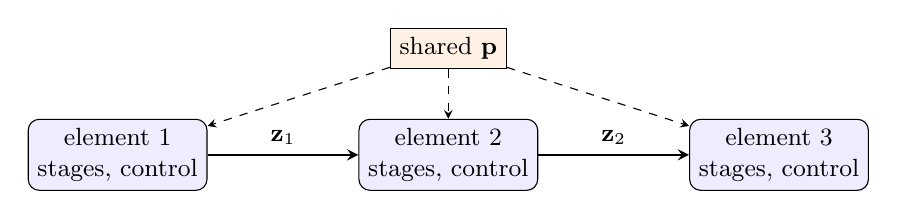
\begin{tikzpicture}[>=stealth,font=\small,blk/.style={draw,rounded corners,align=center,minimum height=.8cm}]
\node[blk,fill=blue!7](a)at(0,0){element 1\\stages, control};
\node[blk,fill=blue!7](b)at(4.2,0){element 2\\stages, control};
\node[blk,fill=blue!7](c)at(8.4,0){element 3\\stages, control};
\draw[->,thick](a)--(b)node[midway,above]{$\mathbf z_1$};
\draw[->,thick](b)--(c)node[midway,above]{$\mathbf z_2$};
\node[draw,fill=orange!10](p)at(4.2,1.35){shared $\mathbf p$};
\draw[->,dashed](p)--(a);\draw[->,dashed](p)--(b);\draw[->,dashed](p)--(c);
\end{tikzpicture}
